\documentclass[11pt]{article}
\usepackage[utf8]{inputenc}
\usepackage[T1]{fontenc}
\usepackage{amsmath}
\usepackage{amsfonts}
\usepackage{amssymb}
\usepackage[version=4]{mhchem}
\usepackage{stmaryrd}
\usepackage{graphicx}
\usepackage[export]{adjustbox}
\graphicspath{ {./images/} }

\begin{document}
\section*{Reading}
Forward Interest Rates

The term structure of interest rates explicitly indicates spot rates-the time value of money from time zero to each prospective point. But it also implicitly indicates forward rates-the time value of money between any two points in time, such as between years 2 and 3 .

\section*{Implied Forward Rates}
Consider an investor holding a one-year zero-coupon bond with a face value of $\$ 100$ and a market value of $\$ 90$. If the investor holds that bond to maturity, the investor's return over the next year will be $11.11 \%$ (a $\$ 10$ gain on a $\$ 90$ position). The investor is contemplating selling the one-year bond immediately and rolling the proceeds into a two-year $\$ 100$ face-value zero-coupon bond, with a market value of $\$ 80$ per $\$ 100$ of face value (offering a yield based on annual compounding of $11.8034 \%)$. If the investor rolled over the full sales price ( $\$ 90$ ) into the two-year bond, the principal amount or face value of the two-year zero-coupon bond that could be purchased would be $\$ 112.50$, which is found as $(\$ 90 / \$ 80) \times \$ 100$. The incremental cash flows of moving from a one-year bond to a two-year bond are shown in Incremental Cash Flows of Moving from a One-Year Bond to a Two-Year Bond.

\begin{center}
\begin{tabular}{|c|c|c|c|}
\hline
 & Year 0 & Year 1 & Year 2 \\
\hline
Current position & $\$ 0$ & $\$ 100$ & $\$ 0$ \\
\hline
Position with rollover & $\$ 0$ & $\$ 0$ & $\$ 112.50$ \\
\hline
Incremental cash flows & $\$ 0$ & $-\$ 100$ & $+\$ 112.50$ \\
\hline
\end{tabular}
\end{center}

The return on the incremental cash flows between years 1 and 2 would be:

$$
(\$ 112.50-\$ 100) / \$ 100=12.50 \%
$$

The incremental cash flows indicate that the investor would have $\$ 100$ less in one year and $\$ 112.50$ more in two years by exchanging the one-year bond for the twoyear bond. The same incremental cash flows can be generated by any investor (in a perfect market) by simply short selling the one-year bond and using all the proceeds to buy the two-year bond.

In this example, $12.50 \%$ is the implied return of investing between periods 1 and 2 in the two-year bond, known as an implied forward rate. An implied forward rate, $F(t, T)$, is the annual return between time $t$ and $T$ (with $T$ ) inferred from the term structure of interest rates.

\section*{Implied Forward Rates with Annual and Continuous Compounding}
The previous section simplified the computation of an implied forward rate by selecting a one-year interval between the starting and ending dates of the forward rate. This section generalizes the computation of the implied forward rates to other time intervals.

Consider an investor weighing two choices:

\begin{enumerate}
  \item Invest for $T$ years at $r_{T}$.
\end{enumerate}

Or

\begin{enumerate}
  \setcounter{enumi}{1}
  \item Invest for a shorter period of time $(t)$ at the rate $r_{t}$ and then reinvest the proceeds into a forward rate, $F(t, T)$ for the remaining $T-t$ years.
\end{enumerate}

In the absence of default risk, these two alternatives should generate identical returns in a perfect market since they each generate riskless proceeds in $T$ years. Setting the future values of $\$ 1$ in $T$ years from both alternatives equals:


\begin{equation*}
\left(1+r_{T}\right)^{T}=\left(1+r_{t}\right)^{t} \times[1+F(t, T)]^{T-t} \tag{1}
\end{equation*}


Solving for $F(t, T)$ generates:


\begin{equation*}
F(t, T)=\left[\left(1+r_{T}\right)^{T} /\left(1+r_{t}\right)^{t}\right]^{1 /(T-t)}-1 \tag{2}
\end{equation*}


The formula is made simpler if the interest rates are expressed using continuous compounding:


\begin{equation*}
e^{r T}=e^{r t} \times e^{F(t, T)(T-t)} \tag{3}
\end{equation*}


Factor the above equation by taking the natural log of each side to produce:


\begin{equation*}
r T=r t+F(t, T)(T-t) \tag{4}
\end{equation*}


Then solve for $F(t, T)$ to produce the general formula (i.e., any $T$ and $t$ with $T>t$ ). The general implied forward rate (based on continuous compounding) is shown in Equation 5.


\begin{equation*}
F(t, T)=\left(r_{T} T-r_{t} t\right) /(T-t) \tag{5}
\end{equation*}


Once again, continuous compounding makes the equation much simpler and intuitive. The intuition is straightforward: receiving $r_{T}$ for $T$ years exceeds $r_{T}$ for $t$ years by $F(t, T)$ per year (i.e., for each year from $t$ to $T$ ). Inserting the previous example with $t=1$ and $T=2$ :

$$
F(1,2)=[(2 \times 11.80434 \%)-(11.11111 \%)] /(2-1)=12.50 \%(\text { rounded })
$$

For the case of $(T-t)=1$ this equation simplifies to:


\begin{equation*}
F(t, T)=r_{T}+\left(r_{T}-r_{t}\right) \times t \tag{6}
\end{equation*}


\section*{The Term Structure of Implied Forward Rates}
Note from Equation 5 that implied forward rates exist for any length time interval (i.e., from any $t$ to any subsequent $T$ ). The two most common choices with which to plot a term structure of forward rates are one year $(T-t=1$ ) and infinitesimal (when $T-t \rightarrow 0$ ). The formula for the implied forward rate for $T-t=1$ is simply: $F(t, T)=\left(r_{T} T-r_{t} t\right)$.

A common structure in interest rate analysis is the term structure of implied forward rates. The term structure of implied forward rates is the relationship between implied forward rates and the starting point of each rate and is often superimposed on the term structure of spot rates. The Term Structure of Single-Period Implied Forward Rates sketches the implied forward rates as lying above the estimated spot rates.

\begin{center}
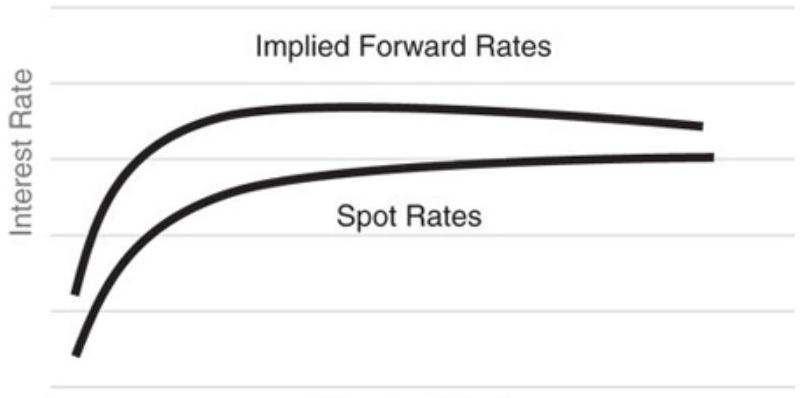
\includegraphics[max width=\textwidth]{2024_04_10_de0b0b0f0220b08f4859g-3}
\end{center}

Time to Maturity

\section*{The Term Structure of Single-Period Implied Forward Rates}
Given the relation for spot and forward rates derived in the previous section, $F(t, T)=\left(r_{T} T-r_{t} t\right) /(T-t)$, it is clear that the forward rate will lie above (below) the spot rate in the case of an upward (downward) sloping spot rate. The gap between the two tends to diminish from left to right. Also, the forward rate tends to "exaggerate" slope changes in the spot rate because the spot is an averaged rate while the forward rate is a marginal rate.

The concepts discussed in this section on implied forward rates serve as a foundation to the discussion of forward contracts in the session entitled Derivatives and Risk-Neutral Valuation.


\end{document}